\chapter{RESULTADOS}\label{cap:resultados}

Os dados desta seção foram coletados na bancada em 02/11/2026, com o firmware descrito no Capítulo~\ref{cap:desenvolvimento}, o indutor instalado, os 12~V ligados e o motor limitado a 32\%. Foram lidos pelo ST-Link, sem alterar o programa, a partir do registro de RAM do próprio firmware (20 amostras por segundo). O \textit{script} \texttt{valida\_com\_dados.py} gera as figuras e os números.

\section{PARTIDA NA BANCADA}

Com os ganhos de projeto ($K_i=0{,}05$) e a haste em repouso, a placa foi reiniciada: durante 2~s o firmware calibra o giroscópio com o motor desligado e, em seguida, arma o controle. A haste sobe de $-36{,}9^\circ$ e, a partir de 6,6~s contados do primeiro registro, fica dentro da faixa de $\pm2^\circ$ em torno do alvo ($0{,}7^\circ$). A saída chegou a no máximo 20,7\%, bem abaixo do limite de 32\%, então o PWM não saturou na partida (Figura~\ref{fig:partida_real}).
\begin{figure}[htbp]
\centering\caption{Partida real após o reset, comparada com a simulação.}\label{fig:partida_real}
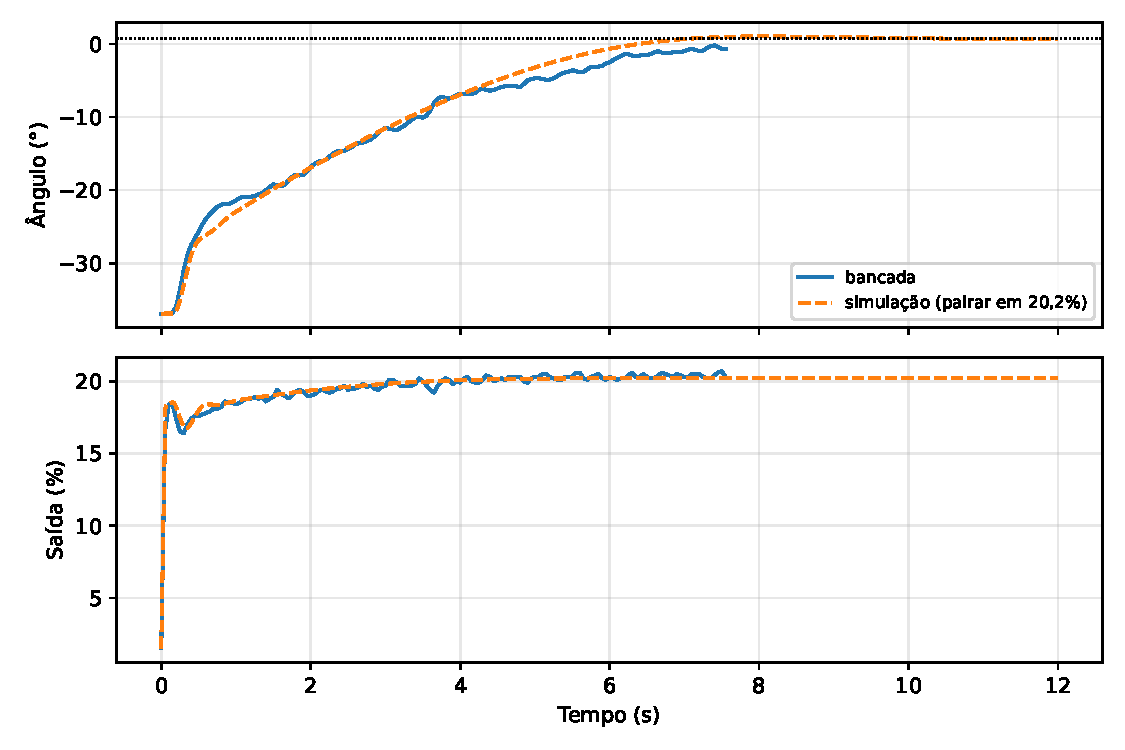
\includegraphics[width=.85\textwidth]{results/partida_real_vs_sim.pdf}
\fonte{Elaborado pelos autores (2026), dados da bancada e simulação com a planta identificada.}
\end{figure}
A simulação, ajustada ao PWM de pairar medido (20,2\%), previu 5,7~s para a mesma partida, ou seja, 14\% menos que o observado; a forma da curva e a saída final coincidem. Em 15,9~s de voo pairando, o ângulo ficou entre $-0{,}1^\circ$ e $1{,}6^\circ$, com média de $0{,}74^\circ$ e desvio padrão de $0{,}33^\circ$, e a saída ficou entre 19,9\% e 20,8\% (média de 20,3\%). A média coincide com o alvo, o que mostra que o controle segue a estimativa de ângulo; a posição física da haste perto da horizontal foi conferida visualmente, sem instrumento.

\section{FILTRO COMPLEMENTAR: COM E SEM FILTRO}

Esta coleta foi feita com a primeira versão do filtro, em que o ângulo em voo vinha só do giroscópio. O ângulo calculado só pelo acelerômetro (``sem filtro'') foi refeito a partir das acelerações X e Z registradas e comparado com o ângulo do firmware. Em repouso, no primeiro registro, os dois diferem em $0{,}2^\circ$ ($-37{,}1^\circ$ contra $-36{,}9^\circ$). Em voo pairando, o acelerômetro tem média de $6{,}4^\circ$, desvio padrão de $8{,}3^\circ$ e extremos de $-9{,}5^\circ$ a $+32{,}7^\circ$, contra desvio de $0{,}33^\circ$ e extremos de $-0{,}1^\circ$ a $1{,}6^\circ$ do ângulo do firmware; a diferença quadrática média entre os dois é de $10{,}0^\circ$ (Figura~\ref{fig:filtro_pairando}). Na partida, a diferença quadrática média em voo foi de $8{,}3^\circ$ (Figura~\ref{fig:filtro_partida}).
\begin{figure}[htbp]
\centering\caption{Ângulo sem filtro (acelerômetro) e do firmware, com a haste pairando.}\label{fig:filtro_pairando}
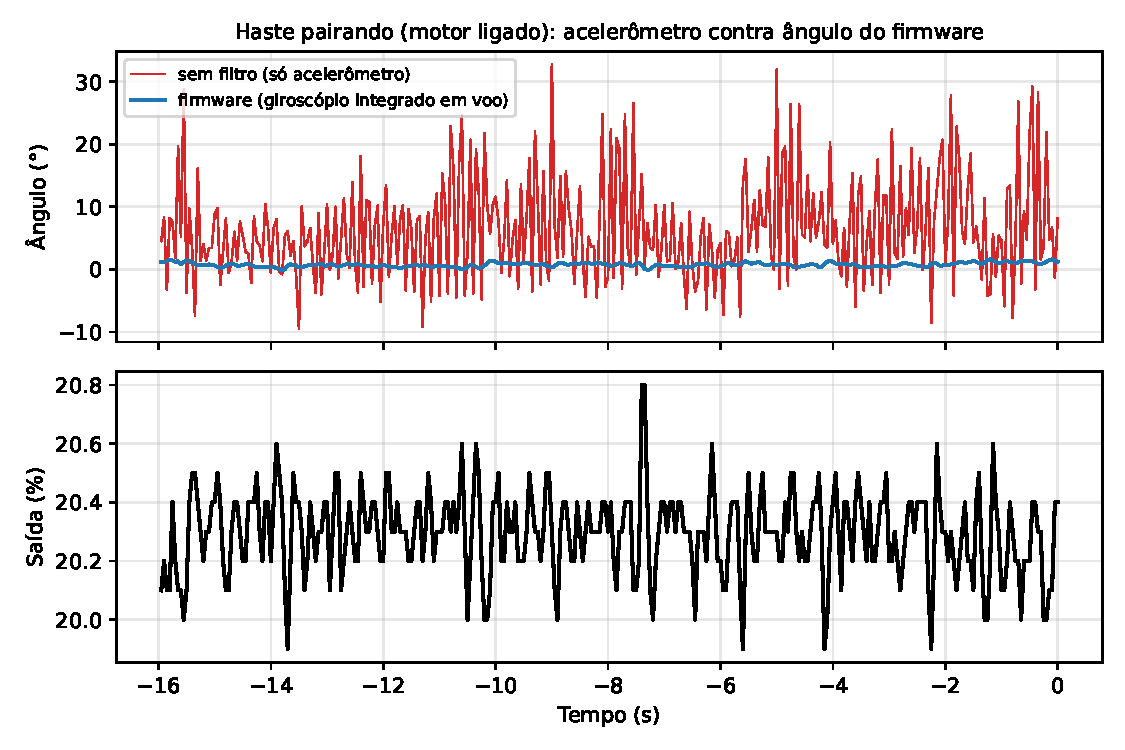
\includegraphics[width=.85\textwidth]{results/filtro_pairando.pdf}
\fonte{Elaborado pelos autores (2026), dados da bancada.}
\end{figure}
\begin{figure}[htbp]
\centering\caption{Ângulo sem filtro (acelerômetro) e do firmware na partida.}\label{fig:filtro_partida}
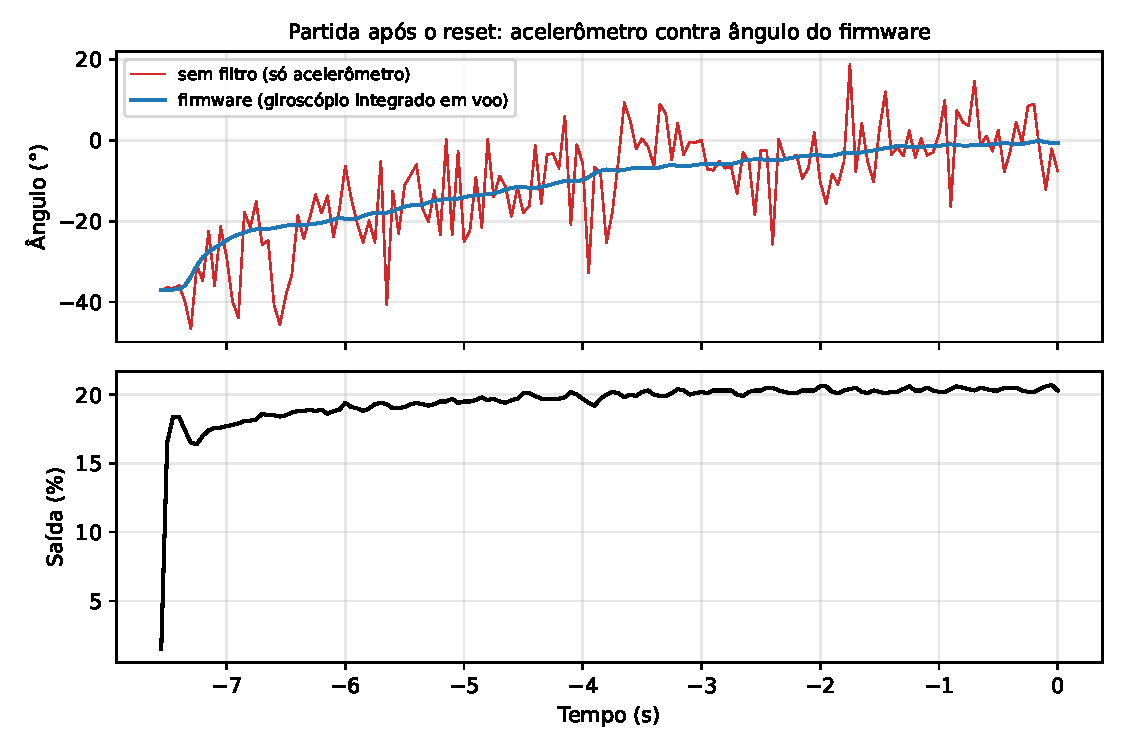
\includegraphics[width=.85\textwidth]{results/filtro_partida.pdf}
\fonte{Elaborado pelos autores (2026), dados da bancada.}
\end{figure}
Usar o acelerômetro direto no controle traria um erro de dezenas de graus e um desvio fixo de cerca de $+6^\circ$. Por isso ele nunca entra direto no controle: na versão final, só corrige o ângulo devagar (Seção~\ref{sec:deriva}). Uma limitação: em voo não há outra referência de ângulo para conferir o giroscópio. A comparação mostra que o acelerômetro não é confiável com a hélice girando, mas não mede o erro do ângulo do firmware. O ensaio de movimento manual com o motor desligado, que mostraria o acelerômetro e o giroscópio concordando, não foi registrado nesta coleta.

\section{PID COM E SEM ANTI-\textit{WINDUP}}

Na bancada, a saída máxima da partida foi de 20,7\%, abaixo do limite de 32\%, de modo que a integração condicional nunca foi acionada. Para conferir, o PID do firmware foi refeito sobre o ângulo e a velocidade medidos, com e sem a integração condicional: as duas saídas foram idênticas, e a saída refeita terminou em 20,4\%, contra 20,3\% da real. Isso valida a reprodução do PID no computador e mostra que, com os ganhos de projeto, o anti-\textit{windup} não altera o comportamento nesta partida. Seu efeito aparece quando a saída satura ou os ganhos são altos, como mostra a simulação (Tabela~\ref{tab:windup}). O firmware final tem uma chave de ensaio (\texttt{aw=0|1} pelo ST-Link), ligada por padrão, que desativa só a integração condicional e mantém o limite do integrador; a comparação na bancada com ela não foi realizada.

\section{DERIVA DO GIROSCÓPIO E CORREÇÃO EM VOO}

Com a primeira versão do filtro (em voo, só giroscópio), a haste segurada no zero físico foi lida pelo acelerômetro em $-1{,}9^\circ$ (média, mediana $-1{,}4^\circ$), enquanto o firmware marcava $+11{,}6^\circ$ após 204~s ligado: 13,5$^\circ$ de erro em 190~s, ou cerca de $4^\circ$/min (Seção~\ref{sec:deriva}). Depois de gravar a versão com correção lenta pelo acelerômetro em voo ($\tau=30$~s, janela de $25^\circ$), a mesma comparação, com a haste pairando sozinha, deu:
\begin{table}[htbp]
\centering\caption{Ângulo do firmware e do acelerômetro em voo, antes e depois da correção.}\label{tab:deriva}
\begin{tabularx}{\textwidth}{Xrrr}
\hline\textbf{Situação} & \textbf{Firmware} & \textbf{Acelerômetro (média)} & \textbf{Diferença}\\\hline
Sem correção, 204~s ligado (haste segurada no zero) & $11{,}6^\circ$ & $-1{,}9^\circ$ & $13{,}5^\circ$\\
Com correção, 130~s ligado (pairando) & $0{,}53^\circ$ & $1{,}4^\circ$ & $0{,}9^\circ$\\
Com correção, 174~s ligado (pairando) & $0{,}77^\circ$ & $2{,}8^\circ$ & $2{,}0^\circ$\\\hline
\end{tabularx}
\fonte{Elaborado pelos autores (2026), dados da bancada em 02/11/2026.}
\end{table}
Com a correção, a diferença caiu de 13,5$^\circ$ para 1 a 2$^\circ$, e o desvio do ângulo do firmware ficou em $0{,}37^\circ$ (extremos de $-0{,}1^\circ$ a $1{,}9^\circ$). A diferença restante é a polarização do acelerômetro em voo, de $+1{,}4^\circ$ a $+2{,}8^\circ$ nestas leituras. O zero físico não foi conferido em voo com um instrumento externo. A única referência externa é a medida feita com a haste parada e segurada no nível do celular, em que o acelerômetro marcou de $-1{,}4^\circ$ a $-1{,}9^\circ$. Assim, o zero físico pode diferir do zero do firmware em alguns graus.

\section{DISTÚRBIOS}

Depois de um empurrão para cima ou para baixo, a haste volta ao alvo, mas com uma leve dificuldade de reassentar exatamente no ângulo desejado. As curvas desses ensaios não foram registradas. As causas prováveis são o integrador, que leva cerca de 7~s para se refazer com $K_i$ pequeno (Seção~\ref{sec:antiwindup}), e a deriva do giroscópio em voo, que na versão inicial chegou a $4^\circ$/min e agora é corrigida lentamente pelo acelerômetro.

\section{ESTABILIDADE DA EXECUÇÃO}

Em 34\,870 ciclos de controle (174~s) da versão final, e em 153\,773 ciclos (768~s) da anterior, não houve nenhuma falha de leitura do MPU6050, nenhum erro da UART e nenhum reinício do I\textsuperscript{2}C; em outras partidas da placa houve um reinício do barramento, recuperado sozinho, sem falha de leitura. A folga mínima de pilha foi de 289, 139 e 127 palavras nas tarefas \texttt{control}, \texttt{cmd} e \texttt{telem} (Seção~\ref{sec:temporal}). O corte por ângulo não foi acionado nesta coleta.

\section{DESEMPENHO TEMPORAL}

Com o contador de ciclos do DWT (Seção~\ref{sec:temporal}), em 34\,870 ciclos (174~s) da versão final: atraso entre a interrupção do TIM2 e o PWM escrito de no máximo 579,5~$\mu$s (média de 557,6~$\mu$s, 99,82\% entre 550 e 600~$\mu$s), 11,6\% do prazo de 5~ms; nenhum tick perdido e nenhum ciclo acima de 5~ms; \textit{jitter} do intervalo entre interrupções de 11,2~$\mu$s no pior ciclo (4\,998,3 a 5\,009,5~$\mu$s); \textit{heap} com 4\,168~bytes livres (menor folga de 3\,472~bytes); Flash de 42~kB. Os valores medidos ficaram dentro das estimativas de projeto.

\chapter{MELHORIA E REFINO}\label{cap:refino}

Os ganhos do PID de projeto ($K_p=0{,}06$, $K_i=0{,}05$, $K_d=0{,}04$, com anti-\textit{windup} por integração condicional) tinham sido escolhidos pela margem de fase (Capítulo~\ref{cap:processo}) e pareciam o estado final. Com o firmware instrumentado e a chave de ensaio do anti-\textit{windup}, foi possível testar outros valores na própria bancada, sem regravar, e escolher com base em medições.

\section{PROCEDIMENTO}

Foram avaliados cinco conjuntos (Tabela~\ref{tab:refino_conj}), escolhidos por margem de fase de pior caso de pelo menos $30^\circ$ no modelo identificado (\texttt{firmware/tools/arm\_margins.py}). Para cada conjunto os ganhos foram escritos na RAM pelo ST-Link, a haste estabilizou por 20~s e foram registradas $N=1\,200$ amostras (60~s a 20~Hz) do ângulo estimado pelo MPU6050, da velocidade e da saída. Em seguida, com os mesmos ganhos, foram aplicados degraus de \textit{setpoint} de $+10^\circ$, $-20^\circ$ e volta ao alvo ($0{,}7^\circ$), com 12~s em cada patamar. O registro de 16~s da RAM é lido várias vezes e costurado pelo índice da amostra (\texttt{firmware/tools/captura\_longa.py} e \texttt{firmware/tools/captura\_degraus.py}); as 60 amostras mais antigas de cada leitura são descartadas porque a leitura não é atômica. Duas coletas de regime foram refeitas porque tiveram perturbações externas (desvios de mais de $3^\circ$ por poucos segundos).
\begin{table}[htbp]
\centering\caption{Conjuntos de ganhos testados.}\label{tab:refino_conj}
\begin{tabularx}{\textwidth}{llllX}
\hline\textbf{Teste} & $K_p$ & $K_i$ & $K_d$ & \textbf{Anti-\textit{windup}}\\\hline
T1 (projeto) & 0,06 & 0,05 & 0,04 & integração condicional\\
T2 & 0,06 & 0,05 & 0,04 & desligado (só limita o integrador)\\
T3 & 0,06 & 0,08 & 0,04 & integração condicional\\
T4 & 0,08 & 0,08 & 0,04 & integração condicional\\
T5 & 0,06 & 0,09 & 0,04 & integração condicional\\\hline
\end{tabularx}
\fonte{Elaborado pelos autores (2026).}
\end{table}

\section{RESULTADOS EM REGIME}

Com a haste pairando, os cinco conjuntos ficaram praticamente iguais (Tabela~\ref{tab:refino_regime}, Figura~\ref{fig:refino_paineis}): erro quadrático médio (RMS) de $0{,}29^\circ$ a $0{,}32^\circ$ e pico a pico de $1{,}7^\circ$ a $2{,}0^\circ$. O ângulo é registrado com resolução de $0{,}1^\circ$, e as diferenças entre testes ficam dentro do ruído. Em regime, portanto, os ganhos testados não se distinguem.
\begin{table}[htbp]
\centering\caption{Regime, $N=1\,200$ amostras (60~s) por teste.}\label{tab:refino_regime}
\begin{tabularx}{\textwidth}{Xrrrr}
\hline\textbf{Teste} & \textbf{Média ($^\circ$)} & \textbf{RMS do erro ($^\circ$)} & \textbf{Pico a pico ($^\circ$)} & \textbf{Máx. $|e|$ ($^\circ$)}\\\hline
T1 & 0,71 & 0,30 & 1,8 & 1,0\\
T2 & 0,60 & 0,31 & 1,8 & 1,1\\
T3 & 0,65 & 0,32 & 2,0 & 1,1\\
T4 & 0,59 & 0,30 & 1,7 & 0,9\\
T5 & 0,62 & 0,29 & 1,8 & 1,0\\\hline
\end{tabularx}
\fonte{Elaborado pelos autores (2026), dados da bancada em 02/11/2026. Erro em relação ao alvo de $0{,}7^\circ$.}
\end{table}
\begin{figure}[htbp]
\centering\caption{Ângulo estimado pelo MPU6050 nos cinco testes, em regime.}\label{fig:refino_paineis}
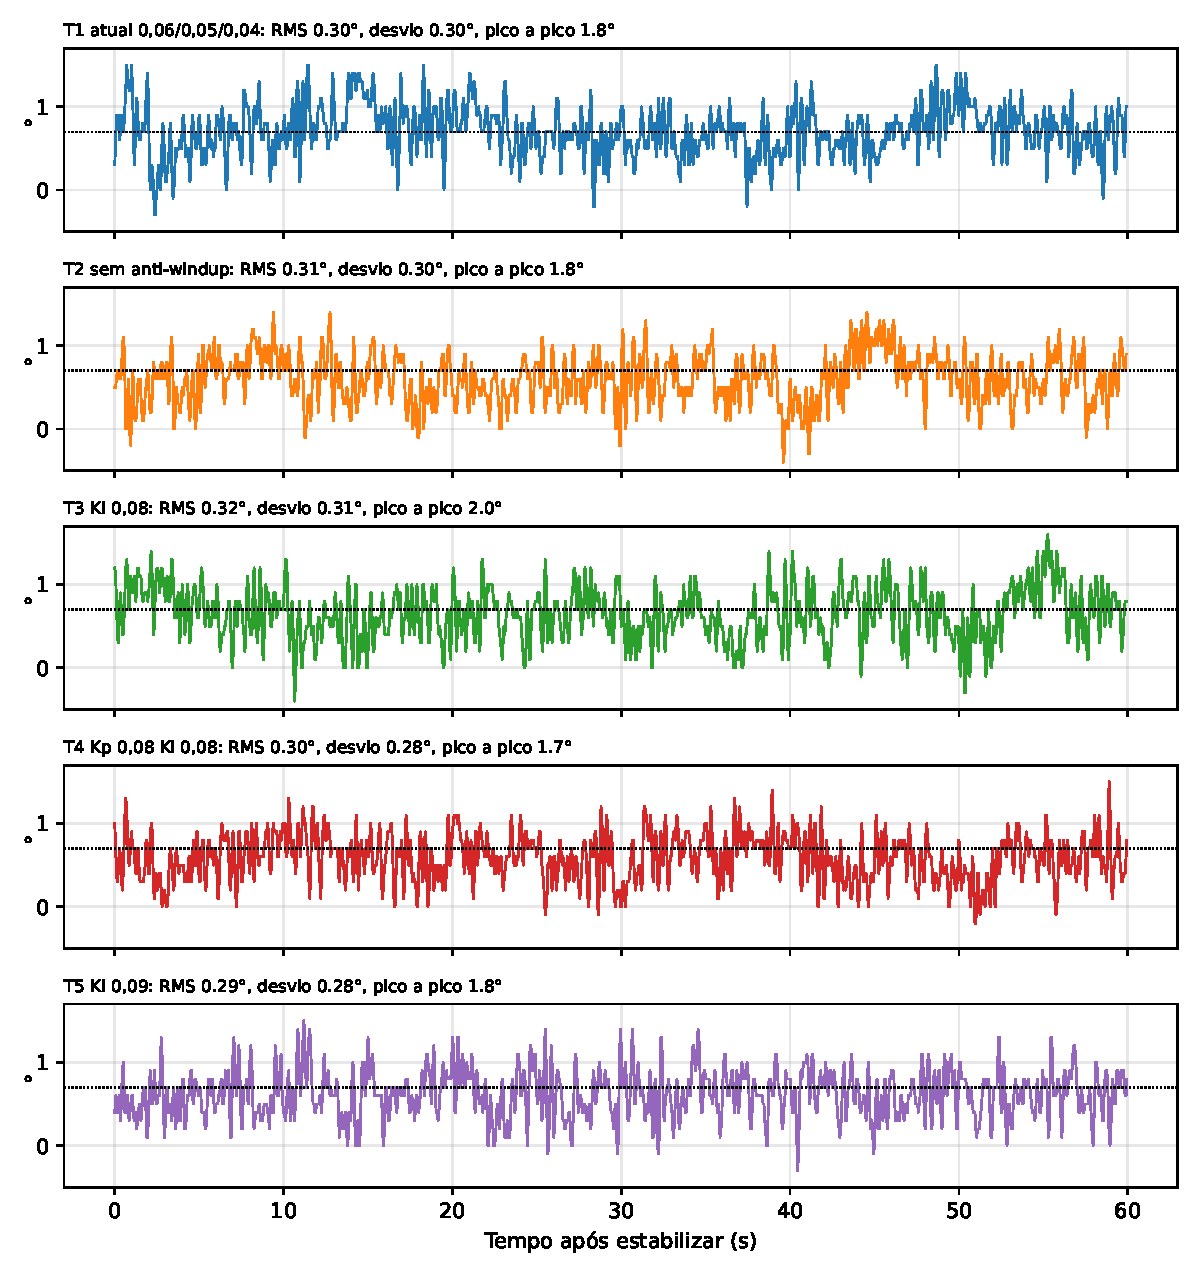
\includegraphics[width=.9\textwidth]{results/refino_paineis.pdf}
\fonte{Elaborado pelos autores (2026), dados da bancada.}
\end{figure}

\section{RESPOSTA A DEGRAUS}

Nos degraus, os conjuntos se separam (Tabela~\ref{tab:refino_degraus}, Figuras~\ref{fig:refino_degraus} e~\ref{fig:refino_degraus_metricas}). O erro acumulado (IAE, integral do módulo do erro, nas três janelas de 12~s) foi de 94,6$^\circ$\,s para o T3 contra 132,0$^\circ$\,s para o T1, 28\% menor. O $K_i$ maior acelera a volta: o tempo para chegar a 90\% do degrau de $-20^\circ$ caiu de 7,5~s (T1) para 4,0~s (T3), e o do retorno ao alvo, de 6,1~s para 3,3~s. O sobressinal do degrau de $+10^\circ$ ficou entre 26\% e 32\% em todos os conjuntos, e portanto não depende dos ganhos testados; reduzi-lo exigiria outra medida, como filtrar o \textit{setpoint}.
\begin{table}[htbp]
\centering\caption{Resposta a degraus de \textit{setpoint}.}\label{tab:refino_degraus}
\begin{tabularx}{\textwidth}{Xrrrrr}
\hline\textbf{Teste} & \textbf{IAE total ($^\circ$\,s)} & \textbf{$t_{90}$ de $+10^\circ$ (s)} & \textbf{$t_{90}$ de $-20^\circ$ (s)} & \textbf{$t_{90}$ da volta (s)} & \textbf{Sobressinal $+10^\circ$ (\%)}\\\hline
T1 & 132,0 & 2,35 & 7,50 & 6,05 & 31,6\\
T2 & 145,4 & 2,90 & 8,00 & 5,55 & 26,6\\
T3 & \textbf{94,6} & 1,95 & 4,00 & 3,25 & 27,2\\
T4 & 109,4 & 1,95 & 4,60 & 4,25 & 26,0\\
T5 & 111,0 & 1,45 & 4,15 & 3,65 & 32,2\\\hline
\end{tabularx}
\fonte{Elaborado pelos autores (2026), dados da bancada em 02/11/2026. Janela de 12~s por degrau.}
\end{table}
\begin{figure}[htbp]
\centering\caption{Resposta aos degraus de \textit{setpoint} nos cinco testes.}\label{fig:refino_degraus}
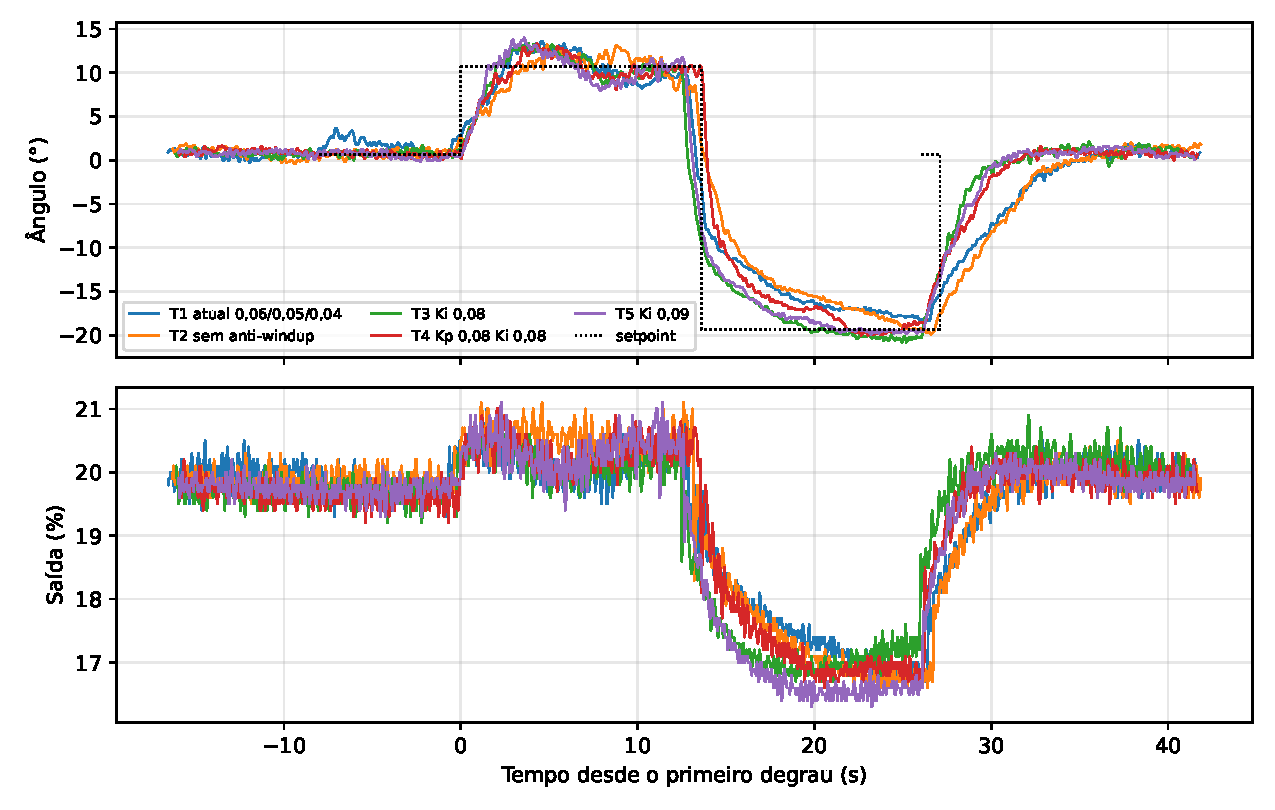
\includegraphics[width=.95\textwidth]{results/refino_degraus.pdf}
\fonte{Elaborado pelos autores (2026), dados da bancada.}
\end{figure}
\begin{figure}[htbp]
\centering\caption{Métricas dos degraus por teste.}\label{fig:refino_degraus_metricas}
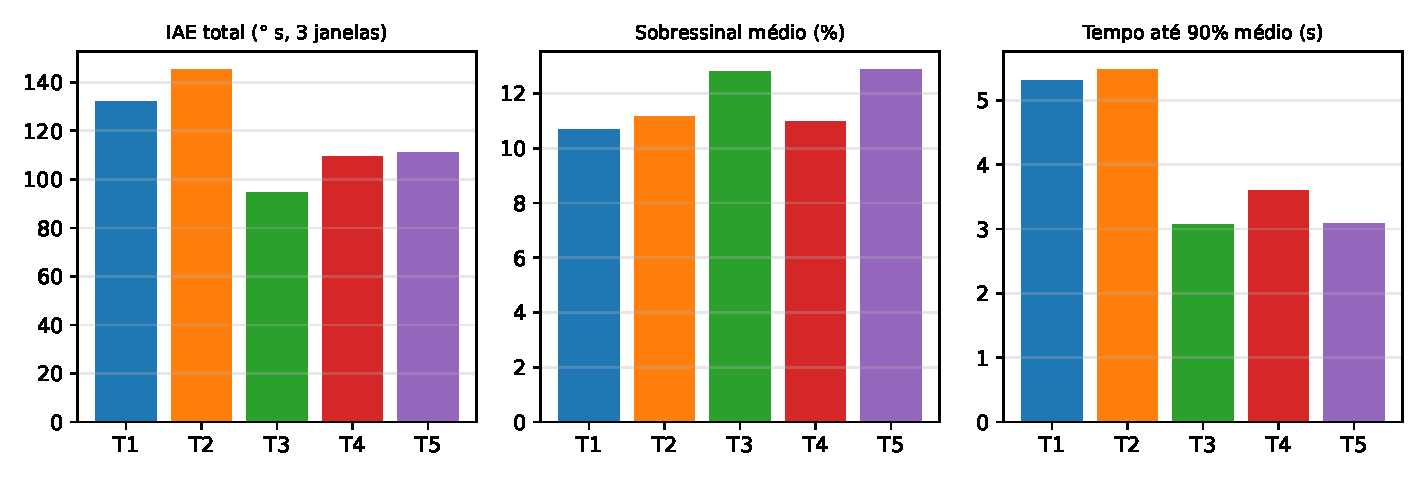
\includegraphics[width=.95\textwidth]{results/refino_degraus_metricas.pdf}
\fonte{Elaborado pelos autores (2026), dados da bancada.}
\end{figure}

\section{ANTI-\textit{WINDUP} NA BANCADA}

A comparação do T1 (com a integração condicional) com o T2 (sem ela) mostrou 9\% a mais de erro acumulado no T2, mas isso não pode ser atribuído ao \textit{windup}: nos degraus, a saída variou de 16,0\% a 21,1\%, sem tocar nos limites de 10\% e de 32\%, de modo que a integração condicional nunca foi acionada. A diferença está dentro da repetibilidade medida: o mesmo conjunto de ganhos do T3, repetido na validação final, deu IAE de 101,5$^\circ$\,s contra 94,6$^\circ$\,s, 7\% de diferença entre execuções. A bancada, nesta faixa de operação, não excita o \textit{windup}; a evidência de que ele importa vem da simulação com ganhos altos e saturação (Seção~\ref{sec:antiwindup}). O anti-\textit{windup} foi mantido ligado por ser uma proteção sem custo.

\section{DECISÃO E ESTADO FINAL}

Foi escolhido o conjunto T3 ($K_p=0{,}06$, $K_i=0{,}08$, $K_d=0{,}04$, com anti-\textit{windup}): menor erro acumulado nos degraus, mesma margem de fase de pior caso do projeto ($32{,}5^\circ$) e regime indistinguível dos demais. T4 e T5 ficaram de 15\% a 17\% acima, pouco mais que o dobro da repetibilidade, e T1 e T2 foram claramente piores. Como $K_i=0{,}08$ passou a ser o valor padrão em \texttt{app\_config.h}, o firmware foi regravado, e o conjunto foi validado de novo (Tabela~\ref{tab:refino_final}).
\begin{table}[htbp]
\centering\caption{Estado final: validação do firmware regravado com $K_i=0{,}08$.}\label{tab:refino_final}
\begin{tabularx}{\textwidth}{Xr}
\hline\textbf{Grandeza} & \textbf{Valor}\\\hline
Regime, $N=1\,200$: média / RMS do erro / pico a pico / máx. $|e|$ & $0{,}67^\circ$ / $0{,}28^\circ$ / $1{,}4^\circ$ / $0{,}7^\circ$\\
Degraus: IAE total & 101,5$^\circ$\,s\\
Degraus: $t_{90}$ de $+10^\circ$ / de $-20^\circ$ / da volta & 2,3~s / 4,25~s / 3,9~s\\
Ciclos, ticks perdidos, atrasos de prazo, cortes por ângulo & 34\,870, 0, 0, 0\\
Latência interrupção até PWM (máx. / média) & 579,5~$\mu$s / 557,6~$\mu$s\\\hline
\end{tabularx}
\fonte{Elaborado pelos autores (2026), dados da bancada em 02/11/2026.}
\end{table}
O estado final do trabalho é, portanto, o conjunto refinado, e não o dos ganhos de projeto: o desempenho em regime é o mesmo, mas o erro acumulado nos degraus é cerca de 28\% menor.
